\documentclass{beamer}
\usepackage{graphicx}

\title{Comparison of Gene Finding Tools in the Context of \textit{Trichoderma} Genomes}
\subtitle{Committee members: Dave Schneider, Tony Kusalik, Matthew Links, Leon Kochian}
\author{Connor Burbridge}
\date{\today}

\begin{document}
\begin{frame}
  \titlepage
\end{frame}

\begin{frame}
  \frametitle{Background: \textit{Trichoderma}}
  What is \textit{Trichoderma}?
  \begin{itemize}
  \item \textit{Trichoderma} is an opportunistic symbiotic fungi, which
    can colonize the roots of plants
  \item \textit{Trichoderma} strains have been shown to provide
    several benefits to the host plant it colonizes, those generally
    being:
    \begin{itemize}
      \item Increased resistance to abiotic and biotic stressors
      \item Facilitating nutrient uptake
      \item Increased germination rates
    \end{itemize}
  \item These benefits have resulted in \textit{Trichoderma} being
    used in manufacturing processes for antibiotics and other materials
  \end{itemize}
\end{frame}

\begin{frame}
  \frametitle{Background: Previous GIFS Work}
  Two strains have been sequenced in previous work within GIFS:
  \begin{itemize}
  \item These strains have been named DC1 and Tsth20
  \item Strains from the prairie regions of Canada, including Alberta
    and Saskatchewan
  \item How exactly do these processes work? Which genes are included
    in these processes?
  \item To answer these questions, both strains were sequenced with
    Illumina and Nanopore technologies
  \end{itemize}
\end{frame}

\begin{frame}
  \frametitle{Research Problem} These sequenced strains offer an
  opportunity to assemble and annotate them:
  \begin{itemize}
  \item Genome assembly is 'relatively' straight-forward
  \item \textbf{However, the choice of a tool for gene finding or
    annotation is uncertain}
  \item There has been relatively little comparative analysis for gene
    finding tools in fungi, and even fewer for \textit{Trichoderma}
  \item \textbf{This raises questions. How do different gene finding
    tools perform in fungi and \textit{Trichoderma} in particular?}
  \end{itemize}
\end{frame}

\begin{frame}
  \frametitle{Project Goal} \textbf{This project aims to evaluate
    several different gene finding tools in the context of
    \textit{Trichoderma} genomes}
  \begin{itemize}
    \item Gene finding tools currently selected are GeneMark-ES and
      Braker2
    \item The selected tools aim to include a mix of \textit{ab
      initio}, evidence-based and hybrid gene finding methods
    \item This list is not final and will include at least one more
      tool for comparison
  \end{itemize}
\end{frame}

\begin{frame}
  \frametitle{Methodology}
  \begin{center}
    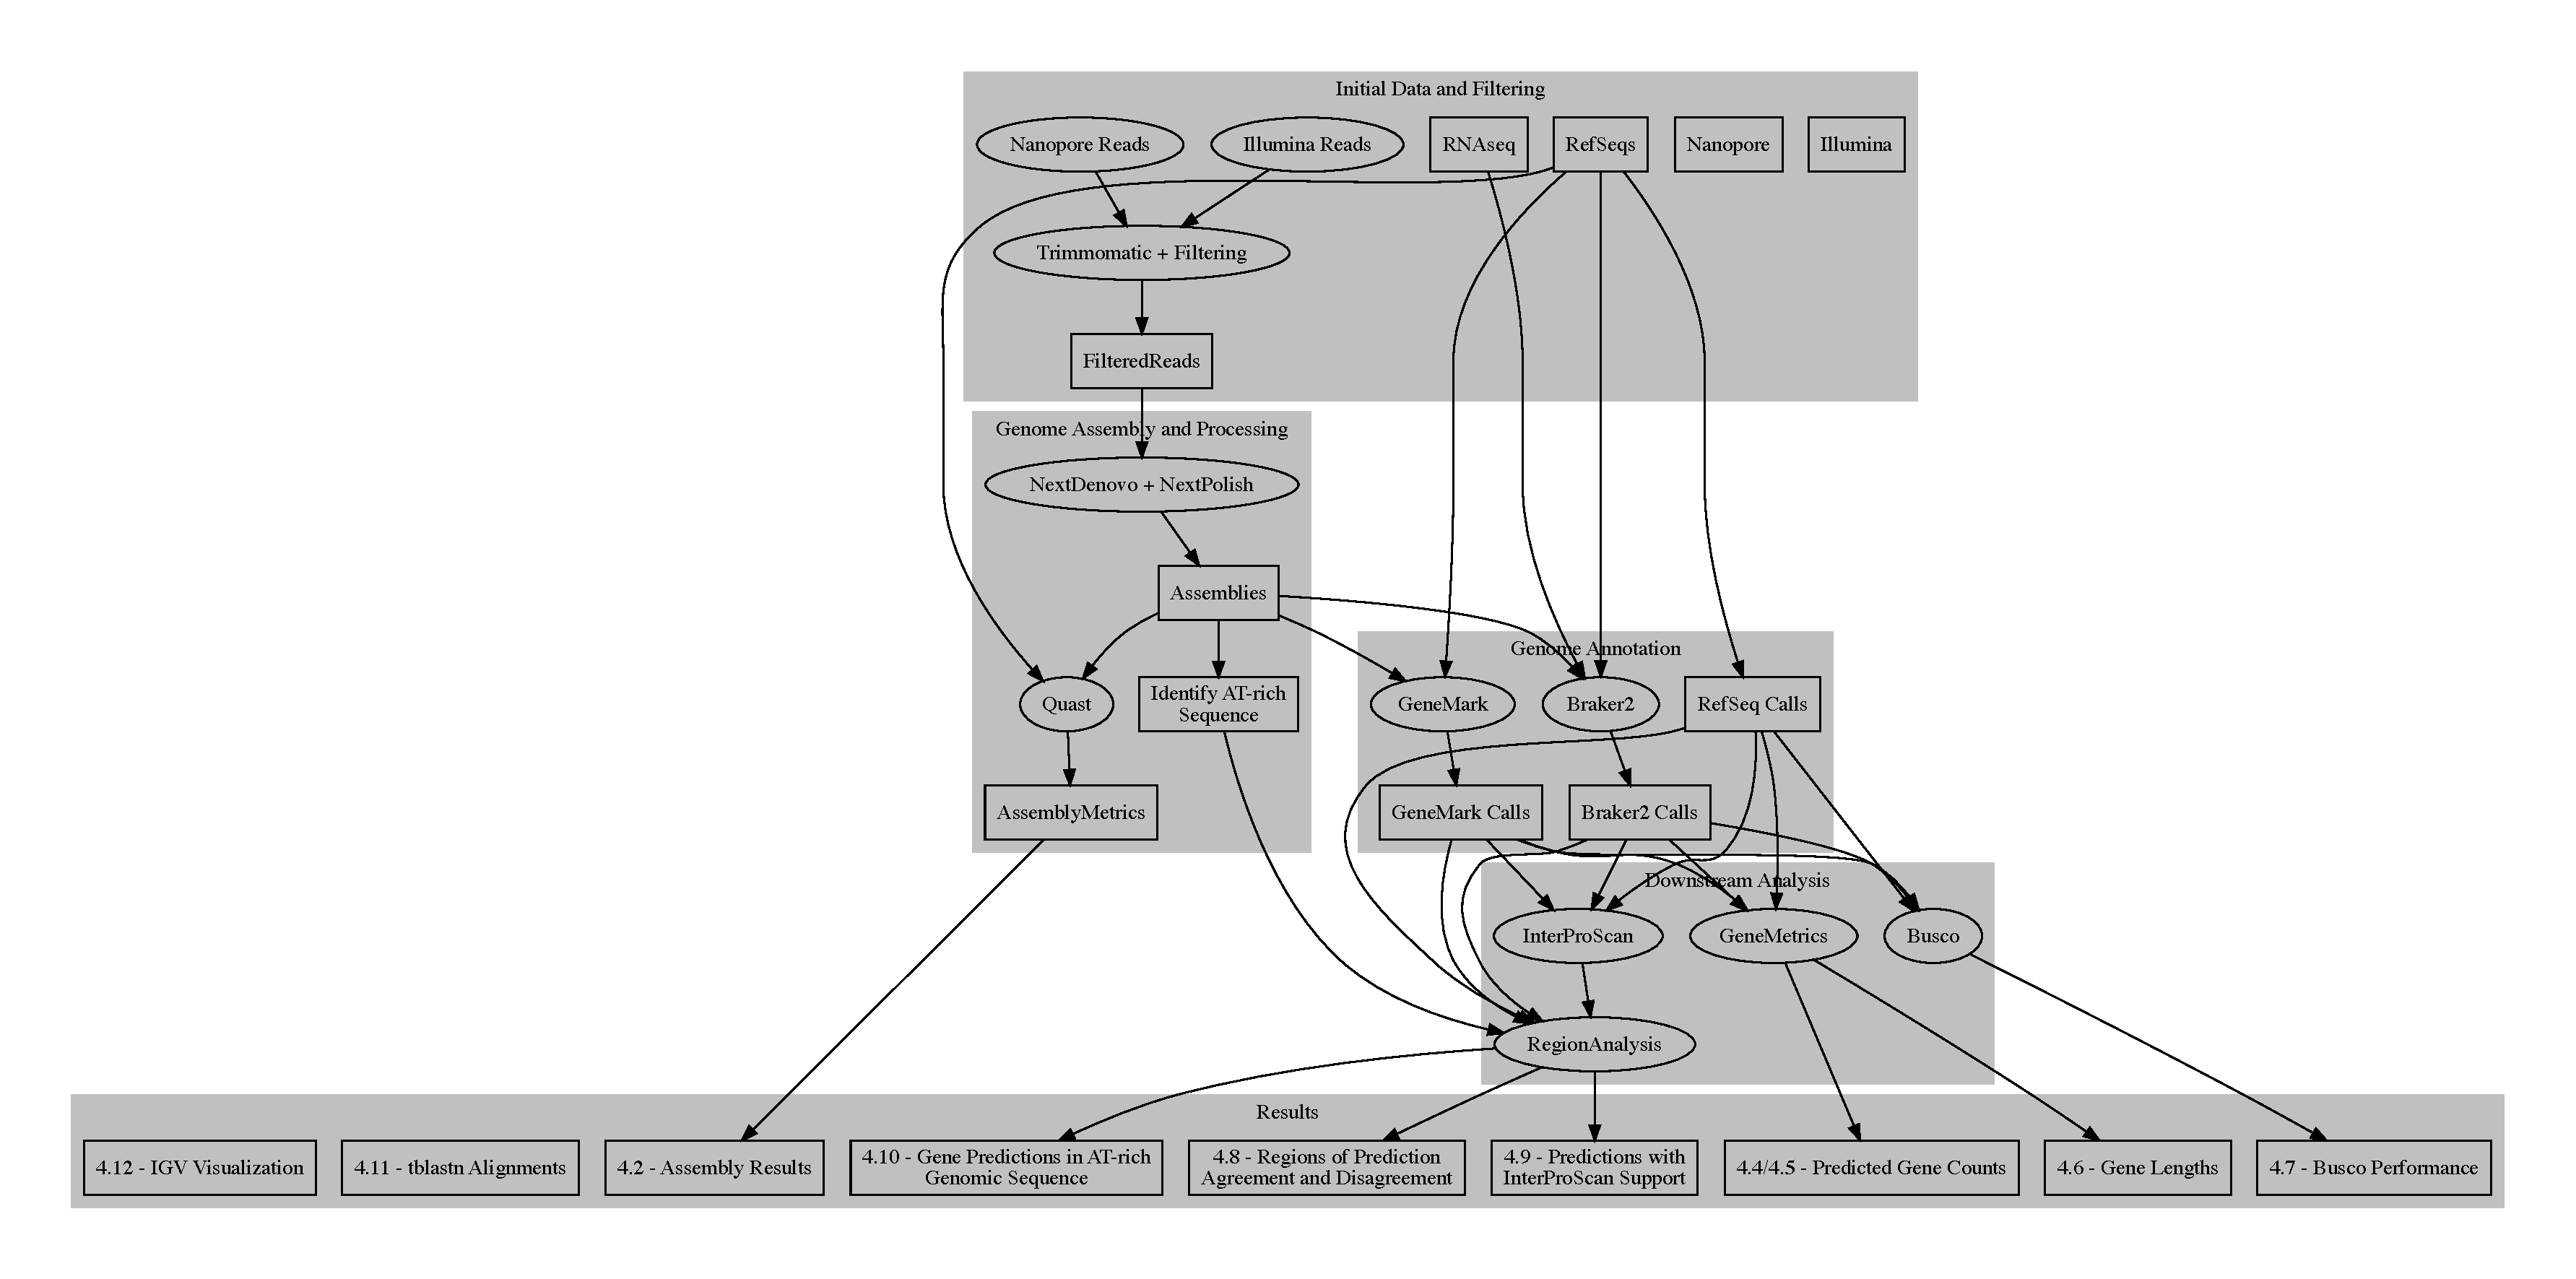
\includegraphics[width=\textwidth]{/Users/cbe453/Desktop/masters/masters/data-flowchart.pdf}
  \end{center}
\end{frame}

\begin{frame}
  \frametitle{Downstream Analysis of Gene Finding Predictions}
  \begin{itemize}
   \item A plan for evaluating and comparing the selected tools needs
     to be developed
   \item Metrics for comparison will include both quantitative and
     qualitative observations

  \end{itemize}
\end{frame}

\begin{frame}

 \frametitle{Quantitative Metrics}
  \begin{itemize}
  \item Total genes predicted
  \item Total transcripts predicted
  \item Genes predicted in repetitive regions
  \item Genes overlapping smallRNAs
  \item Length of gene models predicted
  \item Comparison to genes predicted in other fungal species (Yeast)
  \item Run times and memory usage
  \end{itemize}
\end{frame}

\begin{frame}
  \frametitle{Qualitative Metrics}
  \begin{itemize}
  \item Features of the gene finding tools
  \item Ease of software installation and their dependencies
  \item Ease of use
  \item Popularity among other research
  \end{itemize}
\end{frame}

\end{document}
